%==================================================================%
% Author : Pando Muñoz, Manuel                                     %
%          Sánchez Barreiro, Pablo                                 %
% Version: 1.0, 10/06/2011                                         %
%                                                                  %
% Memoria del Proyecto Fin de Carrera                              %
% Archivo raíz para el capítulo de implementación                  %
%==================================================================%

\chapterheader{Despliegue y aceptación}{Despliegue y aceptación}
\label{chap:despliegue}

\chaptertoc

\section{Despliegue}
\label{sec:despliegue:despliegue}

Para que la aplicación pueda ser usada de un modo cómodo fuera del ambiente de desarrollo se hace necesaria la creación de instaladores. Esto se puede hacer, por ejemplo, con el comando \emph{dpkg} en sistemas Linux derivados de Debian\cite{DEBIAN:2005}, ya que con él se crear archivos .deb. En nuestro caso se han de crear dos instaladores, uno para la aplicación del profesor, y otro para la aplicación de los alumnos.
\newline

En el sistema de archivos, cada carpeta tiene su utilidad, de modo que si, por ejemplo, queremos conocer los logs generados por alguna aplicación sabemos que hemos de buscar en /var/log/, /etc/ para los aspectos de configuraciones, etc.
\newline

Esto es interesante conocerlo para que los archivos que coloque nuestro instalador en el sistema, estén correctamente ubicados, y que se puedan localizar fácilmente, en caso de querer modificarlos o eliminarlos.
\newline

Por ejemplo, la aplicación del alumno, creará en los siguientes directorios, los siguientes ficheros:

\begin{itemize}

    \item {\bfseries /etc/rc2.d:}
    \begin{itemize}
        \item \emph{S88drManhattanDaemon}
    \end{itemize}

    Este fichero contiene un script muy simple que se encarga de iniciar en segundo plano el demonio. Los ficheros en este directorio se ejecutan cuando se entra al segundo nivel de ejecución, en el arranque del sistema.


    \item {\bfseries /usr/bin:}
    \begin{itemize}
        \item \emph{drManhattanAlumno.jar}
        \item \emph{drManhattanAlumno.sh}
        \item \emph{drManhattanDaemon.jar}
    \end{itemize}

    En este directorio se encuentran los ejecutables de las aplicaciones que pueden utilizar todos los usuarios.

    \item {\bfseries /usr/share/applications:}
    \begin{itemize}
        \item \emph{drManhattanAlumno.desktop}
    \end{itemize}

    En nuestro caso se ha utilizado un sistema Ubuntu con el entorno de escritorio GNOME, en ese directorio se guardan las entradas de cada aplicación que se puede ejecutar en GNOME, en archivos de texto dónde se especifica la ruta del ejecutable, el icono del programa, su versión, comentarios, etc.


    \item {\bfseries /usr/share/drManhattanAlumno/iconos:}
    \begin{itemize}
        \item \emph{icono.png}
        \item \emph{envioFichero.png}
        \item \emph{explorar.png}
        \item \emph{fin.png}
    \end{itemize}

    Contiene los datos que no dependen de la arquitectura del sistema, imágenes, sonidos, etc.

    \item {\bfseries /usr/share/menu:}
        \begin{itemize}
            \item \emph{drManhattanAlumno}
        \end{itemize}

    Cada archivo localizado en este directorio contiene la información necesaria para que GNOME pueda crear una entrada en el menú despegable de aplicaciones.


    \item {\bfseries /usr/share/doc/drManhattan-Alumno:}
        \begin{itemize}
            \item \emph{copyright}
            \item \emph{manual.pdf}
        \end{itemize}

    Este directorio contiene documentos relacionados con la aplicación, en este caso los términos de la licencia y el manual de usuario.
\end{itemize}



Una vez que están definidos los archivos y el directorio dónde los ha de colocar el instalador, creamos una carpeta a modo de raíz en la que simulamos el árbol de directorios anterior. Por ejemplo, creamos la carpeta /home/usuario/deb, y dentro de ella creamos /home/usuario/deb/etc/rc2.d/, /home/usuario/deb/usr/bin/, etc y los archivos correspondientes.
\newline

Dentro de la carpeta raíz se ha de crear además de lo anterior, un directorio llamado \lq\lq DEBIAN\rq \rq \ con tres ficheros, \lq\lq control\rq \rq, \lq\lq postinst\rq \rq \ y \lq\lq postrm\rq \rq . En el primero se especifican las características del paquete y los otros dos se ejecutan justo después de instalar el paquete y justo después de desinstalarlo, respectivamente, en nuestro caso actualizan los menús desplegables para que aparezca o desparezca la aplicación.
\newline

Una vez que tenemos todo creado, cambiamos los permisos del directorio raíz y subdirectorios así:

\begin{center}
    \emph{chown root.root -R /home/usuario/deb/}
\end{center}

Después de esto, la orden para empaquetarlo en un fichero .deb es:

\begin{center}
    \emph{dpkg -b /home/usuario/deb /home/usuario/paquete.deb}
\end{center}

Para instalar, teniendo permisos de administrador:

\begin{center}
    \emph{dpkg -i /home/usuario/paquete.deb}
\end{center}


\subsection{Página web}

Para dotar de una mayor visibilidad al proyecto se ha construido una web sencilla, alojada en {\bfseries http://www.alumnos.unican.es/mpm14/} en la que se puede encontrar información, documentación y el código fuente del proyecto. Se han creado además un videotutorial, disponible en la propia web, para poder visualizar el funcionamiento de la aplicación.

\begin{figure}
    \centering
    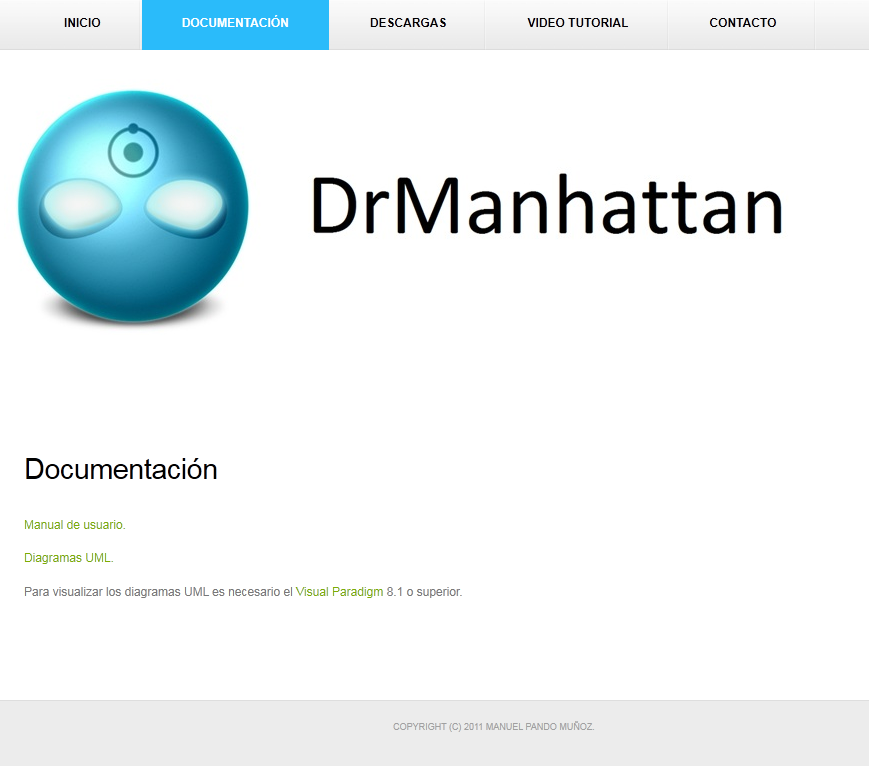
\includegraphics[width=.90\linewidth]{implementacion/web}
    \caption{Página web del proyecto.}
    \label{fig:implementacion:web}
\end{figure}



%Listado de pruebas


\section{Pruebas}
\label{sec:despliegue:pruebas}

Como se comentó en la sección \ref{sec:iteracion1:pruebas} en la que se explicaban las pruebas realizadas durante una iteración, las pruebas han sido combinaciones de acciones, tanto de modo local mientras se desarrollaba, como en los laboratorios de la Facultad con el objetivo de imprimir mayor realismo, tanto en el entorno de ejecución, como en la carga de las aplicaciones.
\newline



\begin{itemize}

    \item Prueba: Intentar conectar a una IP en la que no se está ejecutando la aplicación del profesor.
    \item Objetivo: La aplicación informa del error y permite volver a introducir los datos de conexión.
    \newline

    \item Sin alumnos conectados, enviar fichero de enunciado.
    \item Objetivo: La aplicación del profesor no produce errores y permite seguir ejecutándose.
    \newline

    \item Con un alumno conectado, enviar ficheros de enunciado.
    \item Objetivo: El alumno recibe correctamente el fichero.
    \newline

    \item Con varios alumnos conectados, enviar ficheros de enunciado.
    \item Objetivo: Todos los alumnos reciben correctamente los ficheros.
    \newline

    \item Iniciar prueba sin alumnos conectados.
    \item Objetivo: La prueba queda iniciada, no se admiten nuevas conexiones.
    \newline

    \item Iniciar prueba con varios alumnos conectados.
    \item Objetivo: Desde los computadores de los alumnos no se puede acceder a la red. No se admiten nuevas conexiones.
    \newline


    \item Introducir hora errónea e iniciar prueba.
    \item Objetivo: La aplicación informa del error y la prueba no se inicia.
    \newline

    \item Iniciar prueba temporizada y esperar a que acabe el tiempo.
    \item Objetivo: Cuándo finaliza el tiempo los alumnos recuperan acceso a la red pero no pueden enviar resultados.
    \newline

    \item Iniciar prueba temporizada y finalizar manualmente.
    \item Objetivo: Al finalizar manualmente, cada alumno que esté realizando la prueba recibe un aviso de que ha finalizado. No se pueden enviar ficheros de resultado y se devuelve el acceso a la red.
    \newline


    \item Iniciar prueba normal y finalizar todos los alumnos sin resultados.
    \item Objetivo: Cada alumno deja de poder acceder a la red al iniciar la prueba, cuándo finalizan se les devuelve correctamente el acceso. En la aplicación del profesor se muestran los logs correctos.
    \newline

    \item Iniciar prueba normal y finalizar alumnos sin resultados y alumnos con ellos.
    \item Objetivo: El árbol de directorios se crea correctamente para almacenar los resultados. Los archivos son transferidos correctamente.
    \newline

    \item Iniciar prueba normal y finalizar mientras hay alumnos realizando la prueba.
    \item Objetivo: Cada alumno que esté realizando la prueba recibe un aviso de que ha finalizado. No se pueden enviar ficheros de resultado y se devuelve el acceso a la red.
    \newline


    \item Iniciar prueba normal y reiniciar el computador de un alumno para intentar reconectar sin acabar la prueba.
    \item Objetivo: Al reiniciar un computador con el que se estaba realizando una prueba, la aplicación del alumno reconoce el estado previo y deniega el acceso a la red.
    \newline

    \item Iniciar prueba normal, reiniciar el computador de un alumno, finalizar la prueba e intentar reconectar.
    \item Objetivo: Al reiniciar un computador con el que se estaba realizando una prueba, la aplicación del alumno reconoce el estado previo, intenta reconectarse pero como ya ha finalizado muestra mensaje de error. La red no se desactiva.
    \newline


    \item Iniciar prueba temporizada y reiniciar el computador de un alumno para reconectar antes de que se acabe la prueba.
    \item Objetivo: Al reiniciar, reconecta correctamente y el tiempo restante es correcto.
    \newline

    \item Iniciar prueba temporizada y reiniciar el computador de un alumno para reconectar después de que se acabe la prueba.
    \item Objetivo: Al intentar reconectar no puedo puesto que ya ha finalizado y muestra un error.
    \newline

\end{itemize}


Esta lista contiene las pruebas de integración y validación realizadas, esto es, cuándo se prueba el funcionamiento del sistema completo para comprobar que cumple los requisitos establecidos en la tabla \ref{tabla:requisitos}.
\newline

